\section{Phase 2 - Regression Analysis}

\subsection{Backward Step-wise Analysis}


\begin{center}
\begin{table}
\small
\begin{tabular}{lclc}
\toprule
\textbf{Dep. Variable:}    &   installCount   & \textbf{  R-squared:         } &      0.368   \\
\textbf{Model:}            &       OLS        & \textbf{  Adj. R-squared:    } &      0.368   \\
\textbf{Method:}           &  Least Squares   & \textbf{  F-statistic:       } &      7478.   \\
\textbf{Date:}             & Thu, 07 Dec 2023 & \textbf{  Prob (F-statistic):} &      0.00    \\
\textbf{Time:}             &     20:25:58     & \textbf{  Log-Likelihood:    } & -1.5240e+05  \\
\textbf{No. Observations:} &      128408      & \textbf{  AIC:               } &  3.048e+05   \\
\textbf{Df Residuals:}     &      128397      & \textbf{  BIC:               } &  3.049e+05   \\
\textbf{Df Model:}         &          10      & \textbf{                     } &              \\
\textbf{Covariance Type:}  &    nonrobust     & \textbf{                     } &              \\
\bottomrule
\end{tabular}
%\caption{OLS Regression Results}
\begin{tabular}{lcccccc}
\toprule
                                & \textbf{coef} & \textbf{std err} & \textbf{t} & \textbf{P$> |$t$|$} & \textbf{[0.025} & \textbf{0.975]}  \\
\midrule
\textbf{const}                  &      -0.0401  &        0.003     &   -14.803  &         0.000        &       -0.045    &       -0.035     \\
\textbf{ratingCount}            &       0.5932  &        0.002     &   247.019  &         0.000        &        0.588    &        0.598     \\
\textbf{sizeInMB}               &       0.0299  &        0.002     &    12.388  &         0.000        &        0.025    &        0.035     \\
\textbf{lastUpdateAgeInDays}    &      -0.0737  &        0.002     &   -30.092  &         0.000        &       -0.079    &       -0.069     \\
\textbf{minAndroidVersion\_8}   &      -0.0554  &        0.034     &    -1.616  &         0.106        &       -0.123    &        0.012     \\
\textbf{appAgeInDays}           &       0.0703  &        0.002     &    28.737  &         0.000        &        0.065    &        0.075     \\
\textbf{rating}                 &      -0.0119  &        0.002     &    -5.293  &         0.000        &       -0.016    &       -0.007     \\
\textbf{category\_Productivity} &      -0.0101  &        0.014     &    -0.708  &         0.479        &       -0.038    &        0.018     \\
\textbf{category\_Social}       &      -0.0320  &        0.016     &    -1.957  &         0.050        &       -0.064    &     4.45e-05     \\
\textbf{isInAppPurchases}       &       0.1569  &        0.005     &    30.024  &         0.000        &        0.147    &        0.167     \\
\textbf{minAndroidVersion\_7}   &      -0.1098  &        0.020     &    -5.508  &         0.000        &       -0.149    &       -0.071     \\
\bottomrule
\end{tabular}
\caption{OLS Summary of All Features}
\label{tab:ols-1}
\end{table}
\end{center}


This part of project uses \texttt{statsmodel.OLS} model to estimate a multiple linear regression model. The dependent variable for this model is installCount. Table~\ref{tab:ols-1} is the summary of the first fit for this linear model. From $R^2$, it's clear that the model does not produce a good fit. Further inspection on features is needed. 

Utilizing backward step-wise analysis, \texttt{category\_Productivity} is the first one to remove.\textit{ A small p-value indicates that it is unlikely to observe such a substantial association between the predictor and the response due to chance, in the absence of any real association between the predictor and the response. Hence, if we see a small p-value, then we can infer that there is an association between the predictor and the response}\cite{james2023introduction}. Student's t-tests on each feature's coefficient to the dependent variable are implemented by the model to determine if they significantly contribute to the model. The null hypothesis for each t-test is that the coefficient is equal to zero, meaning it has no effect. Backward step-wise regression requires the operator to remove the feature with the highest p-value until no feature observes p-value that is higher than the significance value. A drawback of this method is that the process is manual. Although I tried to automate the process into a pipeline, the encapsulated library prevented me from doing so.

\begin{center}
    \begin{table}[]
        \centering
        \scriptsize
            \begin{tabular}{cccccccc}
                \hline
                 Removed Feature & p-value & AIC & BIC & R^2 & Adj R^2 & MSE \\
                \hline
                N/A & N/A & 304816.425 & 304923.818 & 0.368 & 0.368 & 4700.899 \\
                category\_Productivity & 0.479 & 304814.926 & 304912.556 & 0.368 & 0.368 & 5223.186 \\
                minAndroidVersion\_8 & 0.105 & 304815.559 & 304903.426 & 0.368 & 0.368 & 5875.877 \\
                category\_Social & 0.052 & 304817.321 & 304895.425 & 0.368 & 0.368 & 6714.950 \\
                \hline
            \end{tabular}
        \caption{Backward Stepwise Analysis}
        \label{tab:backwise}
    \end{table}
\end{center}

Table~\ref{tab:backwise} shows the procedure of backward step-wise analysis. Although the associated features are removed, the model does not observe a higher $R^2$ value. Table~\ref{tab:ols-2} shows the OLS summary of the model after removing features with low associations. Although F-statistics is relatively high, the probability of F-Statistics is 0, which means it fails to reject the hypothesis. Also, the MSE is getting higher after removing redundant features, which is a sign of bad fit.

Considering backward step-wise analysis did not receive positive outcome for this dataset, more regressors need to be considered, for example, random forest regressor. 

\begin{table}
    \centering
    \small
    \begin{center}
        \begin{tabular}{lclc}
        \toprule
        \textbf{Dep. Variable:}       &   installCount   & \textbf{  R-squared:         } &      0.368   \\
        \textbf{Model:}               &       OLS        & \textbf{  Adj. R-squared:    } &      0.368   \\
        \textbf{Method:}              &  Least Squares   & \textbf{  F-statistic:       } &  1.068e+04   \\
        \textbf{Date:}                & Thu, 07 Dec 2023 & \textbf{  Prob (F-statistic):} &      0.00    \\
        \textbf{Time:}                &     21:35:19     & \textbf{  Log-Likelihood:    } & -1.5240e+05  \\
        \textbf{No. Observations:}    &      128408      & \textbf{  AIC:               } &  3.048e+05   \\
        \textbf{Df Residuals:}        &      128400      & \textbf{  BIC:               } &  3.049e+05   \\
        \textbf{Df Model:}            &           7      & \textbf{                     } &              \\
        \textbf{Covariance Type:}     &    nonrobust     & \textbf{                     } &              \\
        \bottomrule
        \end{tabular}
        \begin{tabular}{lcccccc}
                                      & \textbf{coef} & \textbf{std err} & \textbf{t} & \textbf{P$> |$t$|$} & \textbf{[0.025} & \textbf{0.975]}  \\
        \midrule
        \textbf{const}                &      -0.0412  &        0.003     &   -15.422  &         0.000        &       -0.046    &       -0.036     \\
        \textbf{ratingCount}          &       0.5932  &        0.002     &   247.041  &         0.000        &        0.588    &        0.598     \\
        \textbf{sizeInMB}             &       0.0299  &        0.002     &    12.429  &         0.000        &        0.025    &        0.035     \\
        \textbf{lastUpdateAgeInDays}  &      -0.0734  &        0.002     &   -30.001  &         0.000        &       -0.078    &       -0.069     \\
        \textbf{appAgeInDays}         &       0.0702  &        0.002     &    28.752  &         0.000        &        0.065    &        0.075     \\
        \textbf{rating}               &      -0.0118  &        0.002     &    -5.237  &         0.000        &       -0.016    &       -0.007     \\
        \textbf{isInAppPurchases}     &       0.1568  &        0.005     &    30.019  &         0.000        &        0.147    &        0.167     \\
        \textbf{minAndroidVersion\_7} &      -0.1097  &        0.020     &    -5.503  &         0.000        &       -0.149    &       -0.071     \\
        \bottomrule
        \end{tabular}
        \end{center}
        \begin{tabular}{lclc}
        \textbf{Omnibus:}       & 73565.243 & \textbf{  Durbin-Watson:     } &      1.995   \\
        \textbf{Prob(Omnibus):} &    0.000  & \textbf{  Jarque-Bera (JB):  } & 2705960.736  \\
        \textbf{Skew:}          &    2.156  & \textbf{  Prob(JB):          } &       0.00   \\
        \textbf{Kurtosis:}      &   25.072  & \textbf{  Cond. No.          } &       11.3   \\
        \bottomrule
        \end{tabular}
        %\caption{OLS Regression Results}
        
    \caption{OLS Summary of Remaining Features}
    \label{tab:ols-2}
\end{table}

\subsection{Random Forest Regressor}

Random forest regressor is used for a better outcome than linear regression. To begin with, a initial training of the \texttt{RandomForestRegressor} is executed. From the initial training, the feature importance can be obtained.

Figure~\ref{fig:rfg} shows the feature importances of the initial run. For all 13 features used in initial build, after the $6^{th}$ feature, importances plumbed. Therefore keeping only the features whose importance is higher than 0.05. 

\begin{figure}
    \centering
    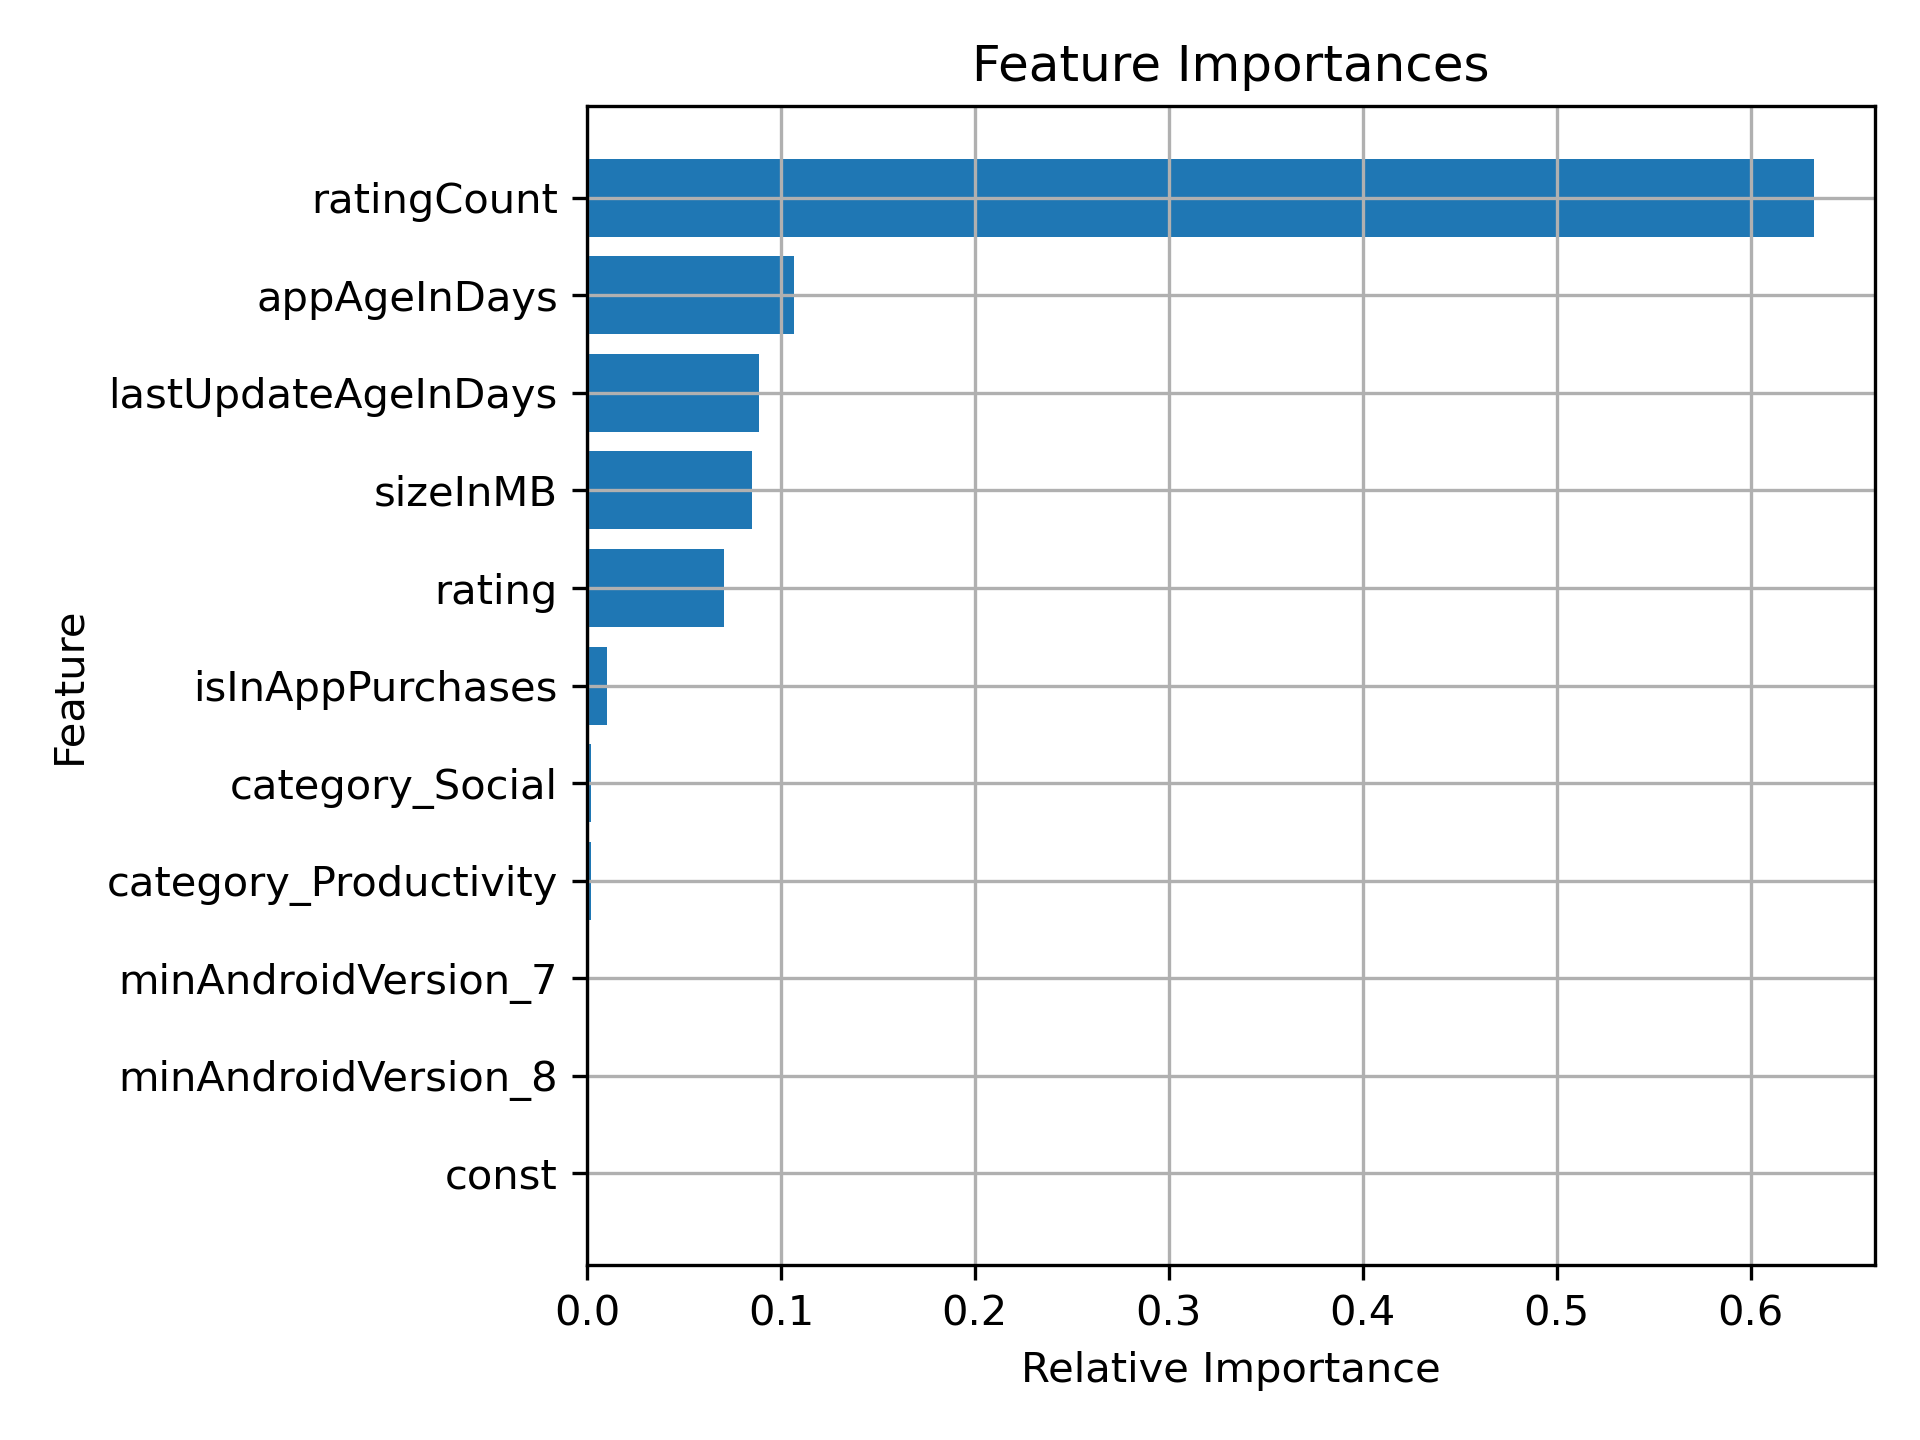
\includegraphics[width=1\linewidth]{docs//assets/regressor_feature_importances.png}
    \caption{Random Forest Regressor - Feature Importance}
    \label{fig:rfg}
\end{figure}

After setting threshold as 0.05, another training of the regressor based on the new feature matrix with only important features is executed. In order to prevent over-fitting, K-Fold cross-validation (10 folds) is used to evaluate the model, calculating MSE for each fold.

\begin{table}[h]
\centering
\scriptsize
\begin{tabular}{|c|c|c|c|c|c|c|c|c|c|c|}
\hline
\textbf{Fold 1} & \textbf{Fold 2} & \textbf{Fold 3} & \textbf{Fold 4} & \textbf{Fold 5} & \textbf{Fold 6} & \textbf{Fold 7} & \textbf{Fold 8} & \textbf{Fold 9} & \textbf{Fold 10} \\
\hline
0.42 & 0.42 & 0.41 & 0.44 & 0.43 & 0.46 & 0.42 & 0.42 & 0.44 & 0.40 \\
\hline
\end{tabular}
\caption{10-fold Cross Validation Mean Squared Error Scores}
\label{tab:kfold_scores}
\end{table}

The final result of the random forest regressor is in table~\ref{tab:rfg-results}, compared to the results in table~\ref{tab:ols-2}, the $R^{2}$ is significantly increased, meaning that this tree-based model is a better fit for this dataset. Seemingly unusual negative AIC and BIC values are also accepted\cite{burnham2003model}, and provides an apparently better fit than linear regression model. Low AIC and BIC indicates a preferred model. As observed from both table~\ref{tab:kfold_scores} and table~\ref{tab:rfg-results}, the MSE is very low. K-fold prevents possible over-fitting, that's the reason testing MSE in the table is similar to training data.



\begin{table}[ht]
\centering
\begin{tabular}{|l|l|l|l|l|}
\hline
$R^2$ & Adj $R^2$ & AIC       & BIC       & MSE  \\ \hline
0.58  & 0.58   & -27065.07 & -27023.19 & 0.43 \\ \hline
\end{tabular}
\caption{Final Regression Model Results}
\label{tab:rfg-results}
\end{table}

\begin{figure}
    \centering
    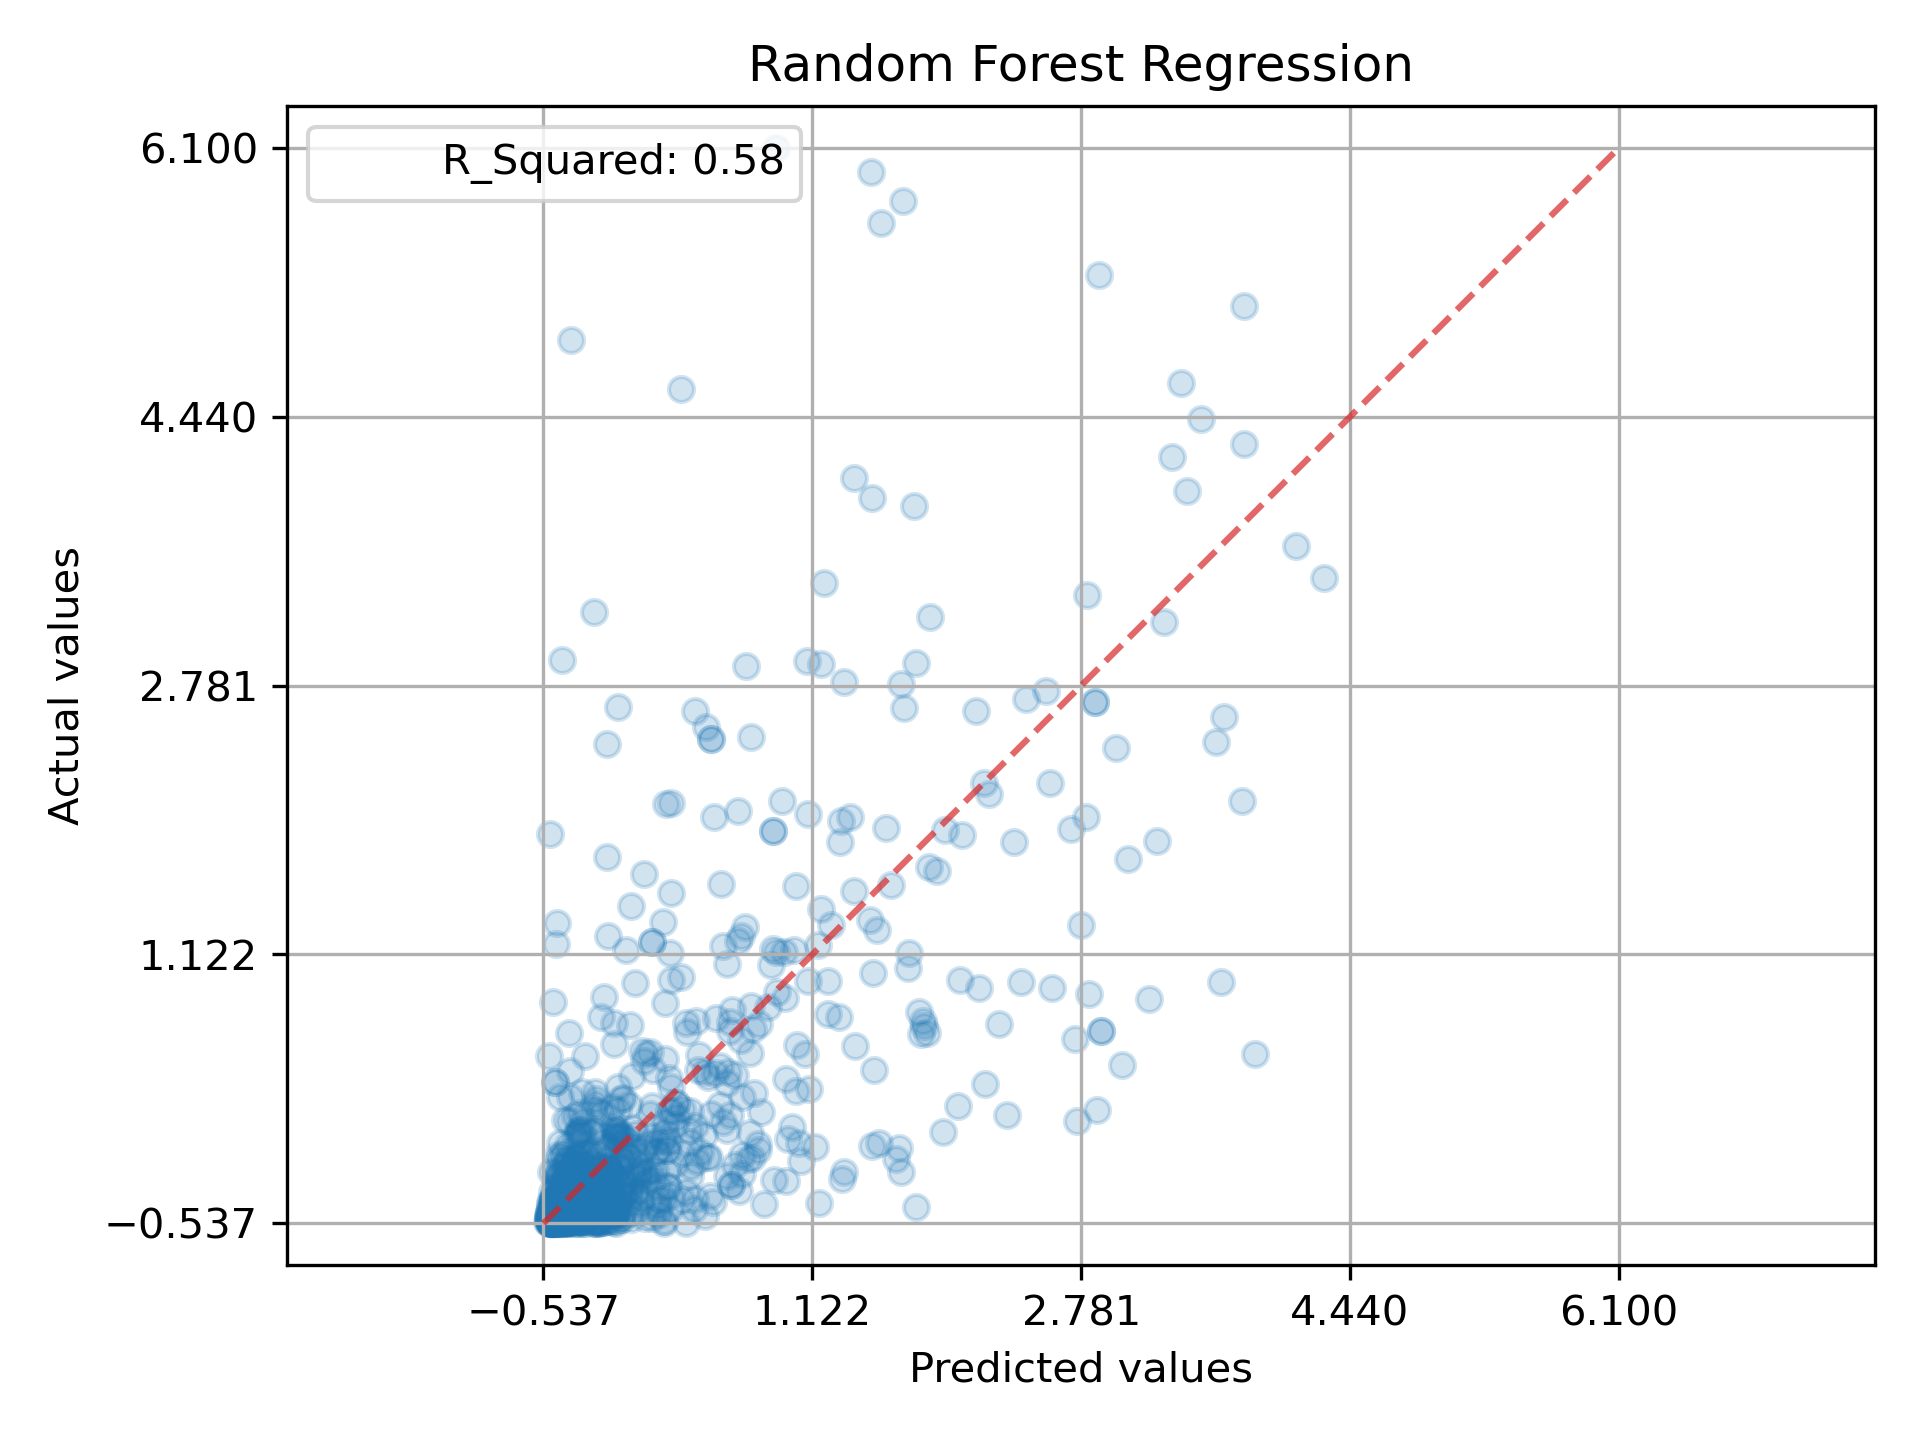
\includegraphics[width=1\linewidth]{docs//assets/regressor_prediction_error.png}
    \caption{Actual vs Predicted Values - Random Forest Regressor}
    \label{fig:rfg-scatter}
\end{figure}

Figure~\ref{fig:rfg-scatter} shows the plot of actual and predicted values via random forest regressor. Although scattered and radiactive, a better fit than linear regression is observed. Figure~\ref{fig:rfg-ci} shows the first 100 samples' predicted \texttt{installCount} and actual \texttt{installCount}. Most of values are with the boundaries of confidence interval, which indicates a good fit by the random forest regression model.

\begin{figure}
    \centering
    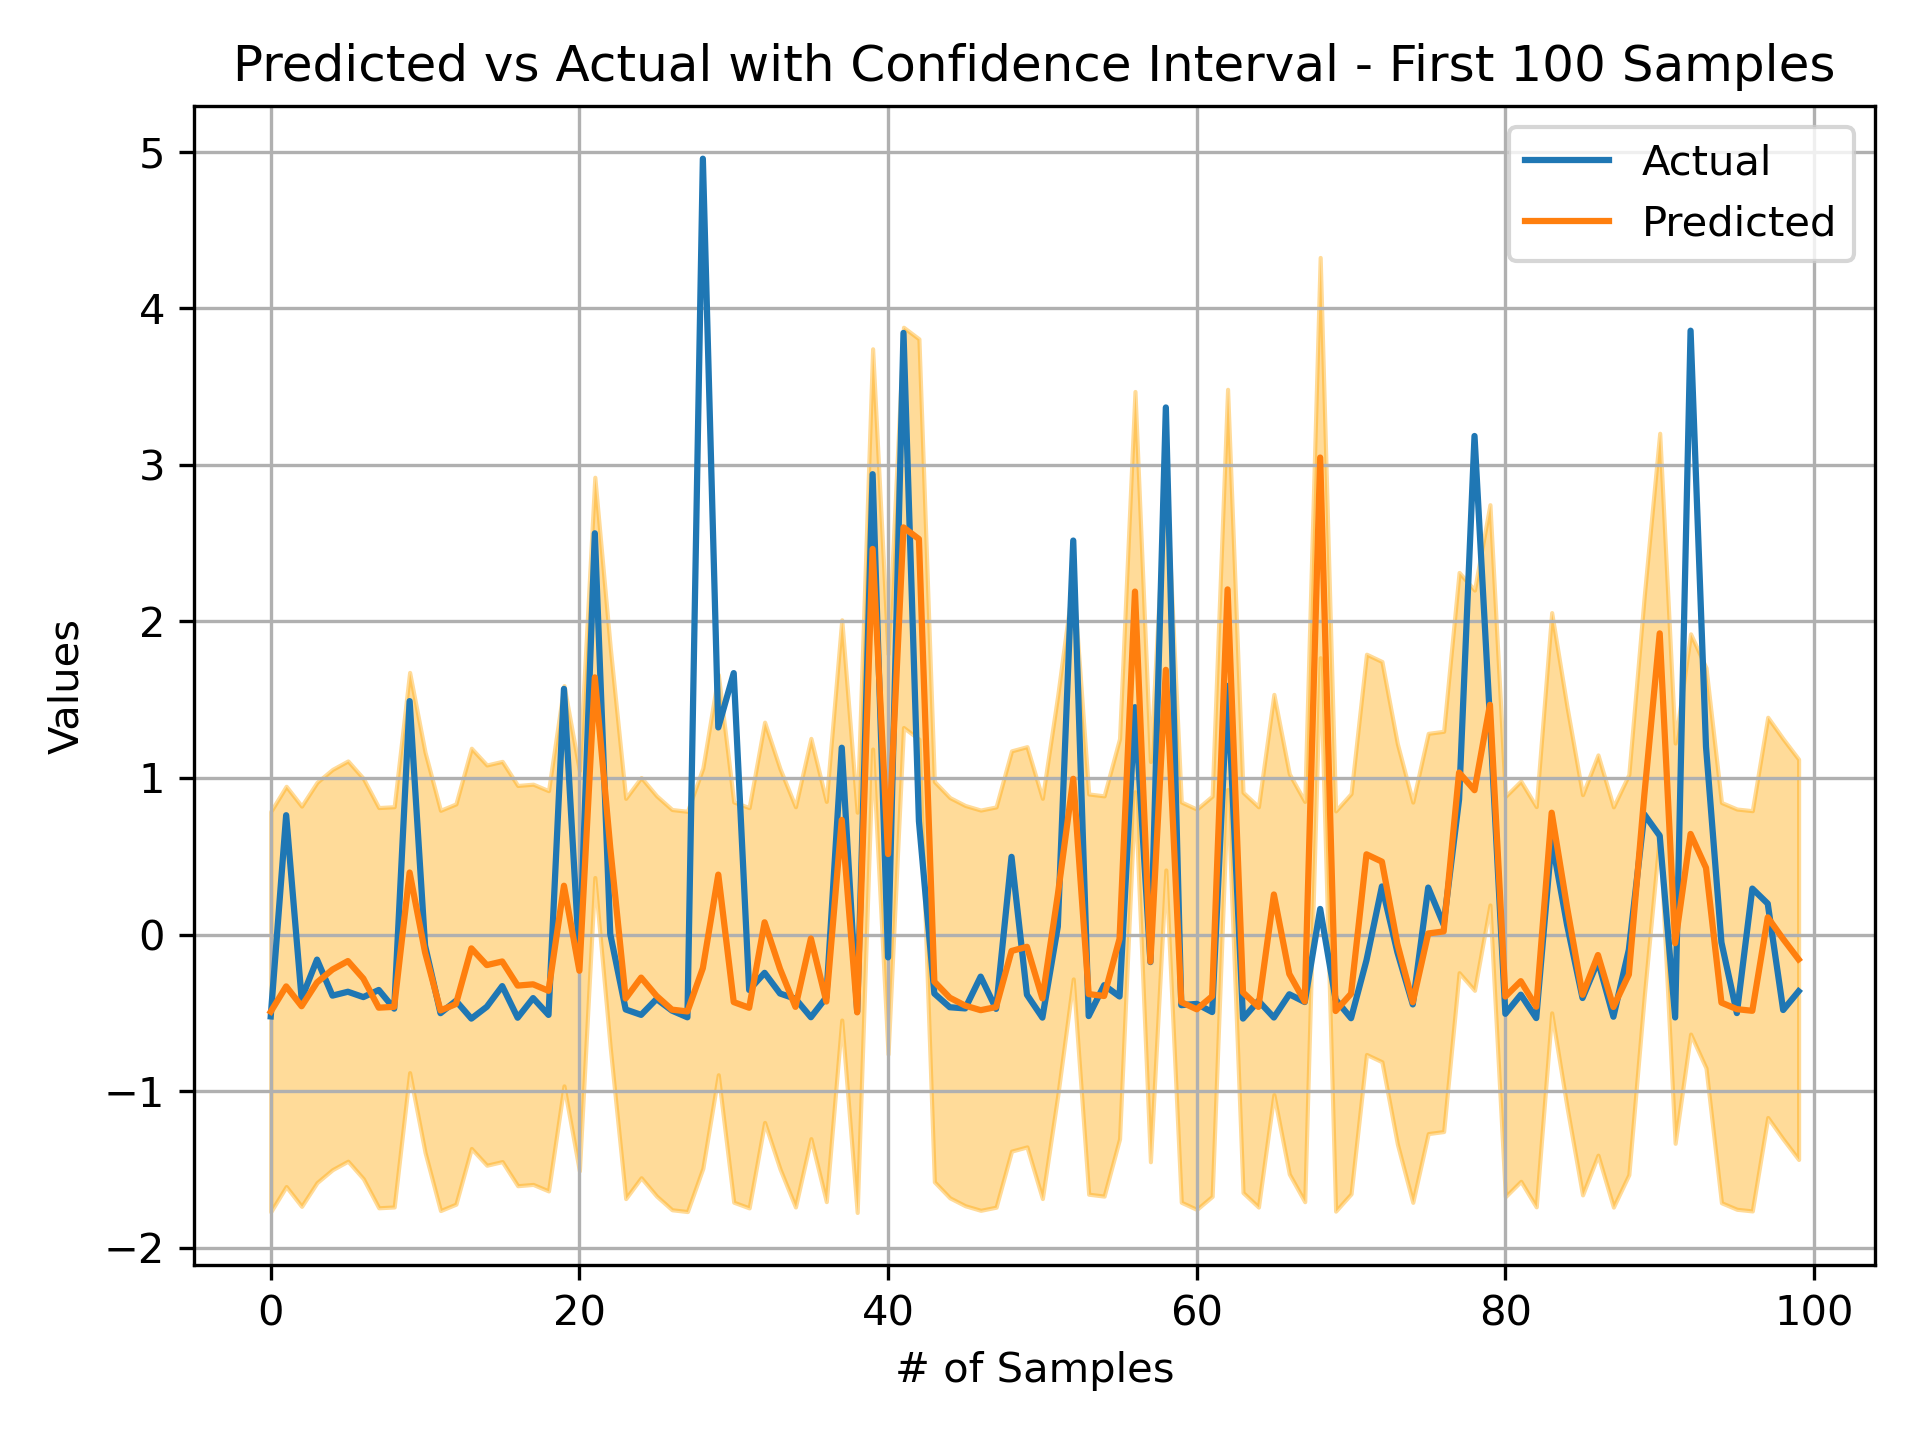
\includegraphics[width=1\linewidth]{docs//assets/regressor_predicted_vs_actual.png}
    \caption{Predicted vs Actual with Confidence Interval}
    \label{fig:rfg-ci}
\end{figure}

\subsection{Conclusion}

In conclusion, the regression analysis conducted in Phase 2 of this project reveals significant insights into the prediction of \texttt{installCount}. Initially, a multiple linear regression model using the \texttt{statsmodel.OLS} was employed. Despite the high F-statistics, the model exhibited a low $R^2$ value and an increasing MSE, indicating a poor fit. The backward step-wise analysis, intended to improve the model by removing features with high p-values, did not yield a significant increase in the $R^2$ value or a decrease in MSE.

In response to these limitations, the project pivoted to a Random Forest Regressor, which demonstrated a marked improvement over the linear model. The tree-based approach resulted in a higher $R^2$ value, indicating a better fit for the dataset. The implementation of K-Fold cross-validation addressed potential overfitting issues, as evidenced by the low and consistent MSE scores across different folds.

The graphical analysis, including the plot of actual versus predicted values and the comparison within confidence intervals, further substantiates the Random Forest Regressor's effectiveness. These visuals show a more accurate and reliable prediction of installCount compared to the linear regression model.

Overall, the transition from a linear to a tree-based model in this analysis underscores the importance of model selection in data analysis. The Random Forest Regressor, with its ability to handle a large number of features and its resistance to overfitting, proved to be a more suitable choice for predicting installCount, offering both higher accuracy and reliability.